\documentclass[11pt]{article}

\usepackage[a4paper,margin=1in]{geometry}
\usepackage[T1]{fontenc}
\usepackage{lmodern}
\usepackage{amsmath,amssymb}
\usepackage{booktabs}
\usepackage{graphicx}
\usepackage{xcolor}
\usepackage{hyperref}
\usepackage{microtype}
\usepackage{parskip}
\usepackage{float}
\usepackage{enumitem}
\usepackage{array}
\usepackage{mdframed}

\graphicspath{{figures/}}

\hypersetup{
  colorlinks=true,
  linkcolor=blue!60!black,
  urlcolor=blue!60!black,
  citecolor=blue!60!black,
  hypertexnames=false
}

\definecolor{grpoblue}{HTML}{1565C0}
\definecolor{reinforcered}{HTML}{C62828}
\definecolor{lightbg}{HTML}{F7F9FC}

\newmdenv[
  backgroundcolor=lightbg,
  linecolor=black!20,
  linewidth=0.8pt,
  roundcorner=4pt,
  innertopmargin=8pt,
  innerbottommargin=8pt,
  innerleftmargin=10pt,
  innerrightmargin=10pt,
  skipabove=8pt,
  skipbelow=8pt
]{examplebox}

\title{\textbf{CS 285 Assignment 4: LLM RL Report}}
\author{Xiaolei Chu \\ Student ID: 3038525739}
\date{Spring 2026}

\begin{document}
\maketitle

\section*{Experimental Context}
All figures and numbers below come from the actual exported W\&B runs included with the submission. The four required runs were:
\begin{itemize}[leftmargin=1.4em]
\item \texttt{format\_copy + GRPO}
\item \texttt{format\_copy + GR-REINFORCE}
\item \texttt{math\_hard + GR-REINFORCE} using the final passing rerun (\texttt{math\_hard\_reinforce\_rerun3})
\item \texttt{math\_hard + GRPO}
\end{itemize}

The five extra ablation runs were all additional \texttt{format\_copy + GRPO} runs with one hyperparameter changed at a time:
\texttt{ppo\_epochs=1}, \texttt{kl\_coef=0.01}, \texttt{kl\_coef=0.20}, \texttt{clip\_eps=0.10}, and \texttt{minibatch\_size=24, grad\_accum\_steps=1}.

\section{Question 1: Approximate KL}
Let
\[
\Delta(a) = \log \pi_{\mathrm{ref}}(a \mid s) - \log \pi_{\theta}(a \mid s)
\]
for a sampled token \(a \sim \pi_\theta(\cdot \mid s)\) at decoding state \(s\). The homework uses
\[
\hat{k}(a) = e^{\Delta(a)} - \Delta(a) - 1
\]
as the sampled-token KL penalty.

The key identity is
\[
e^{\Delta(a)} = \frac{\pi_{\mathrm{ref}}(a \mid s)}{\pi_\theta(a \mid s)}.
\]
Taking expectation under the current policy gives
\[
\mathbb{E}_{a \sim \pi_\theta}\!\left[e^{\Delta(a)}\right]
= \sum_a \pi_\theta(a \mid s) \frac{\pi_{\mathrm{ref}}(a \mid s)}{\pi_\theta(a \mid s)}
= \sum_a \pi_{\mathrm{ref}}(a \mid s)
= 1.
\]
Also,
\[
\mathbb{E}_{a \sim \pi_\theta}\!\left[\Delta(a)\right]
= \mathbb{E}_{a \sim \pi_\theta}\!\left[\log \pi_{\mathrm{ref}}(a \mid s) - \log \pi_\theta(a \mid s)\right]
= - \mathrm{KL}\!\left(\pi_\theta(\cdot \mid s)\,\|\,\pi_{\mathrm{ref}}(\cdot \mid s)\right).
\]
Therefore,
\[
\mathbb{E}[\hat{k}(a)]
= \mathbb{E}[e^{\Delta(a)}] - \mathbb{E}[\Delta(a)] - 1
= 1 - (-\mathrm{KL}) - 1
= \mathrm{KL}\!\left(\pi_\theta(\cdot \mid s)\,\|\,\pi_{\mathrm{ref}}(\cdot \mid s)\right).
\]
So \(e^{\Delta}-\Delta-1\) is an unbiased sampled-token estimator of the exact KL divergence.

This estimator is attractive because it only needs the log-probability of the \emph{sampled token}, which we already compute during rollout and update. By contrast, the exact token-level KL requires a full sum over the vocabulary:
\[
\mathrm{KL}\!\left(\pi_\theta(\cdot \mid s)\,\|\,\pi_{\mathrm{ref}}(\cdot \mid s)\right)
= \sum_{a \in \mathcal V}
\pi_\theta(a \mid s)
\log \frac{\pi_\theta(a \mid s)}{\pi_{\mathrm{ref}}(a \mid s)}.
\]
For this homework, a typical \texttt{math\_hard} rollout can have \(64\) completions per training step and up to \(512\) generated tokens. With a vocabulary on the order of \(1.5 \times 10^5\), the dense tensor needed for exact KL would be about
\[
64 \times 512 \times 150{,}000 \approx 4.9 \times 10^9
\]
logit values. Even in half precision that is roughly \(10\) GB just to hold one large distribution tensor, before counting activations, model weights, and optimizer state. The sampled-token estimator avoids that memory and compute cost entirely.

\section{Question 2: Implementation Order and One Bug}
\textbf{Implementation order.} I followed the suggested dependency order from the homework:
\begin{enumerate}[leftmargin=1.6em]
\item \texttt{compute\_per\_token\_logprobs}, \texttt{build\_completion\_mask}, and \texttt{approx\_kl\_from\_logprobs}
\item \texttt{iter\_minibatches}
\item \texttt{compute\_group\_advantages} and \texttt{maybe\_normalize\_advantages}
\item \texttt{Reinforce.update}
\item \texttt{GRPO.update}
\end{enumerate}
This was the right order in practice: once token-level log-probs and masks were correct, the rollout buffer and the two update rules became much easier to reason about.

\textbf{One bug/confusion point.} The most important bug I hit was in \texttt{compute\_group\_advantages}. My first version treated a near-zero reward standard deviation as a batch-level failure case:
\[
\text{if any group has } \sigma_g < \varepsilon,\ \text{return all-zero advantages.}
\]
That was wrong. It meant one ``flat'' prompt group could zero out the learning signal for the \emph{entire} rollout batch. On \texttt{format\_copy}, this happened late in training when some prompt groups already had identical rewards, and it caused intermittent dead updates. The correct fix was to apply the fallback \emph{per group}: normalize the stable groups normally, and set only the unstable groups to zero with a \texttt{torch.where}-style mask.

The other conceptual confusion point was the completion mask indexing. The log-prob tensor has shape \([B, L-1]\) because position \(t\) scores token \(x_{t+1}\), so the first completion token lives at mask index \(\texttt{prompt\_input\_len} - 1\), not at \(\texttt{prompt\_input\_len}\). Once I wrote that down explicitly, the rest of the alignment issues became much easier.

\section{Question 3: GR-REINFORCE vs.\ GRPO on \texttt{math\_hard}}
Figure~\ref{fig:math_compare} compares the two \texttt{math\_hard} runs. Over the first 200 training iterations, both runs start from the same pretrained baseline of \(22.66\%\) boxed-answer exact match, but GRPO pulls ahead steadily.

\begin{figure}[H]
  \centering
  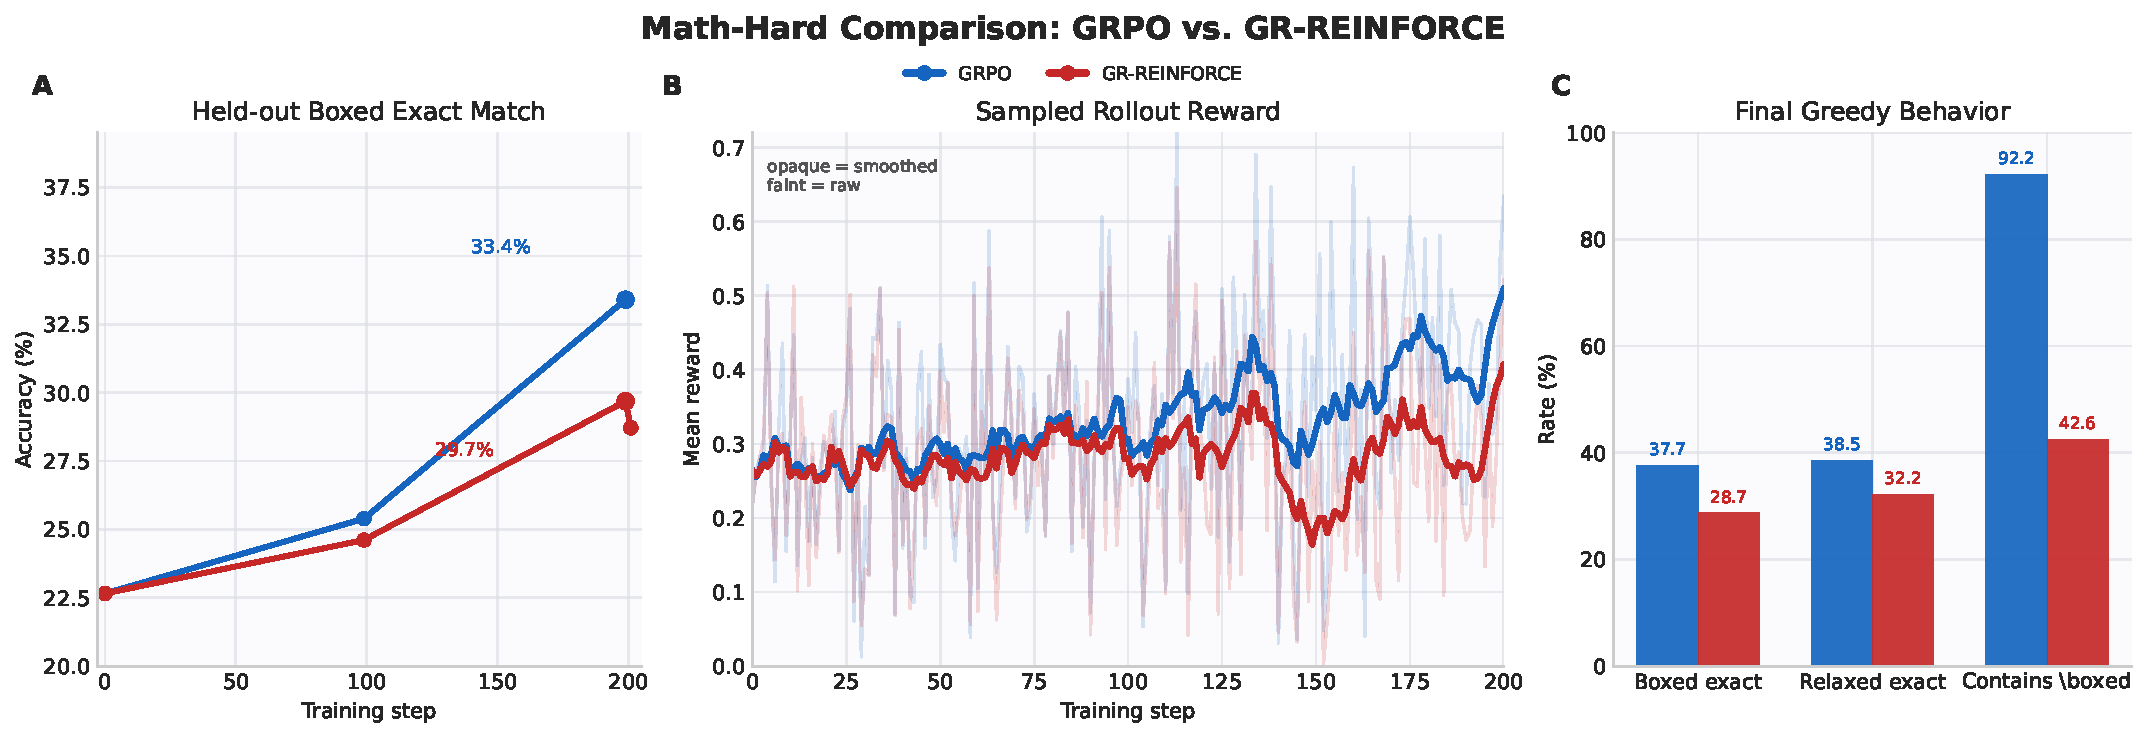
\includegraphics[width=\textwidth]{math_compare.pdf}
  \caption{Comparison of the two \texttt{math\_hard} runs. Panel A shows boxed-answer exact match over the first 200 iterations; Panel B shows sampled rollout reward; Panel C shows the final greedy behavior that matters most for evaluation.}
  \label{fig:math_compare}
\end{figure}

\begin{table}[H]
\centering
\caption{Key \texttt{math\_hard} metrics from the actual W\&B runs.}
\label{tab:math_compare}
\resizebox{\textwidth}{!}{%
\begin{tabular}{@{}lcccccc@{}}
\toprule
\textbf{Run} & \textbf{Step 0} & \textbf{Step 99} & \textbf{Step 199} & \textbf{Final boxed exact} & \textbf{Final boxed-pattern rate} & \textbf{Relaxed-only gap} \\
\midrule
GR-REINFORCE & 22.66\% & 24.61\% & 29.69\% & 28.71\% @ step 201 & 42.58\% & 3.52\% \\
GRPO         & 22.66\% & 25.39\% & 33.40\% & 37.70\% @ step 501 & 92.19\% & 0.78\% \\
\bottomrule
\end{tabular}
}
\end{table}

There are two takeaways.

First, GRPO is better on the actual homework metric. By step 199, GRPO reaches \(33.40\%\) boxed exact while GR-REINFORCE reaches \(29.69\%\). GRPO then continues climbing to \(37.70\%\) by the end of its longer run, whereas the final passing GR-REINFORCE rerun finishes at \(28.71\%\) on step 201.

Second, the difference is \emph{not} just ``higher sampled reward.'' In fact, the GR-REINFORCE run ends with a higher \emph{sampled} rollout reward (\(0.522\) at step 200) than the GRPO run's final-batch reward in the summary, yet its greedy boxed-answer accuracy is worse. The explanation is visible in Panel~C: GR-REINFORCE relies much more on the relaxed last-number parser and emits the required \verb|\boxed{}| format much less consistently. Its final boxed-pattern rate is only \(42.58\%\), compared with \(92.19\%\) for GRPO. The relaxed-minus-boxed gap is also much larger for GR-REINFORCE (\(3.52\%\) vs.\ \(0.78\%\)). In other words, GR-REINFORCE is often ``numerically close'' on sampled rollouts without consistently producing the exact greedy format that the evaluator parses.

This comparison is especially interesting because the provided commands are nearly matched:
\begin{itemize}[leftmargin=1.4em]
\item same task and model
\item same \texttt{batch\_size=8}, \texttt{group\_size=8}, \texttt{minibatch\_size=8}, \texttt{grad\_accum\_steps=8}
\item same learning rate and KL coefficient
\end{itemize}
The main algorithmic difference is that GRPO reuses the same rollout data with \texttt{ppo\_epochs=2} and a clipped PPO-style objective, while GR-REINFORCE makes one on-policy pass. The W\&B curves show that this extra reuse is not just a theoretical benefit: on \texttt{math\_hard}, it converts into noticeably better boxed-answer behavior under greedy evaluation.

\section{Question 4: GRPO Ablations on \texttt{format\_copy}}
All six \texttt{format\_copy + GRPO} runs eventually reached \(100\%\) eval exact match, so the informative differences are in \emph{how fast} they learn and what the diagnostics say about the update dynamics.

\begin{figure}[H]
  \centering
  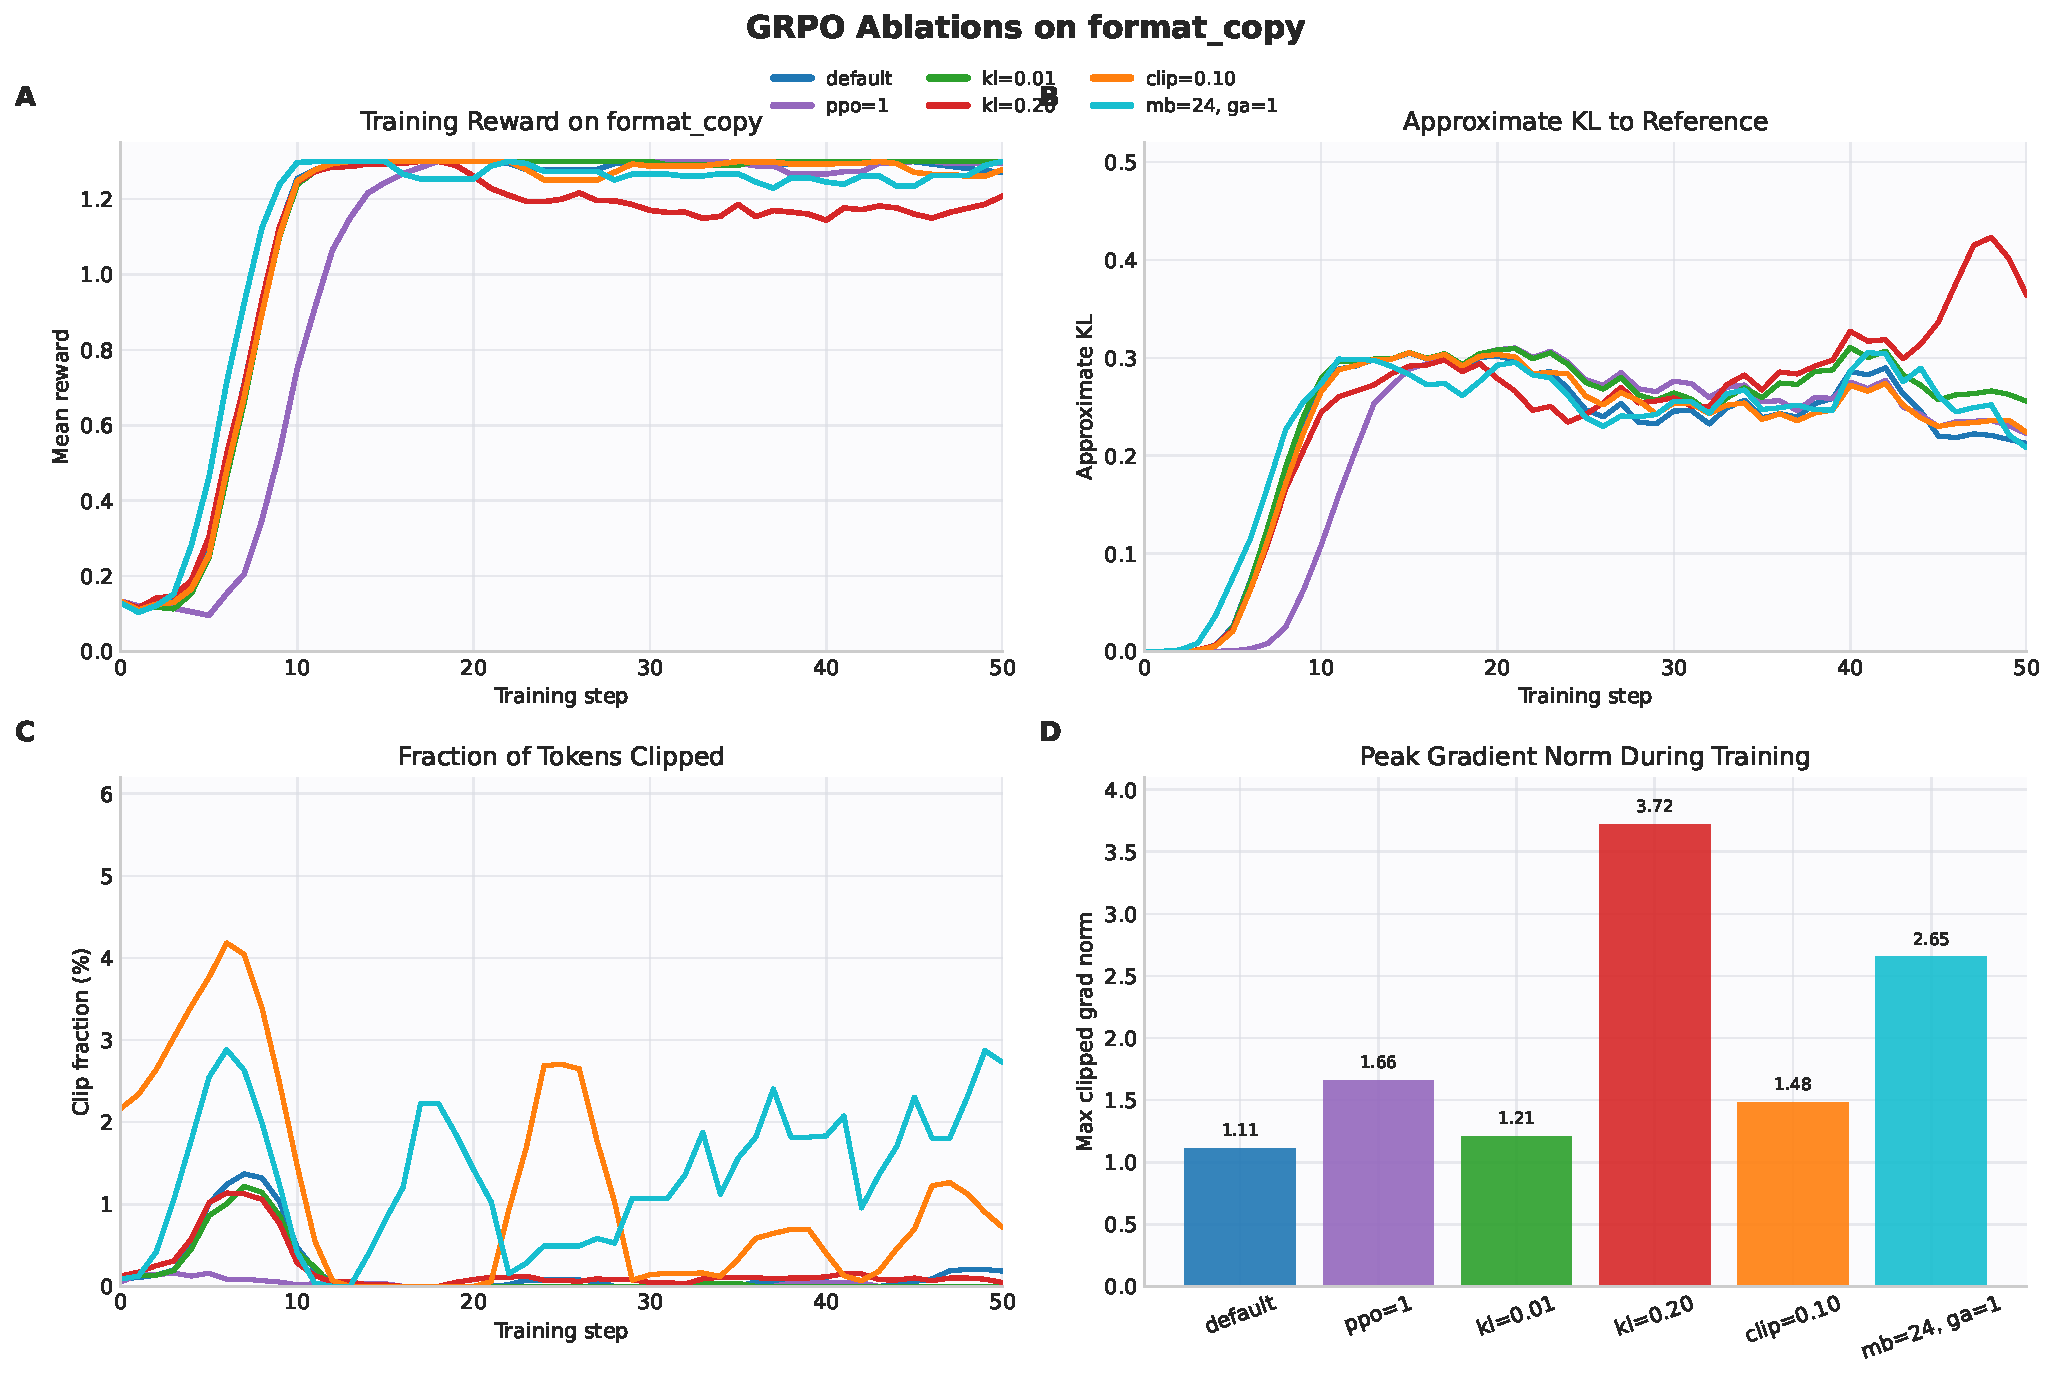
\includegraphics[width=\textwidth]{ablation_compare.pdf}
  \caption{The five GRPO ablations plus the default \texttt{format\_copy} GRPO run. The easiest task metric saturates for all runs, so the most useful signals are reward speed, KL growth, clipping behavior, and gradient spikes.}
  \label{fig:ablation_compare}
\end{figure}

\begin{table}[H]
\centering
\small
\caption{Summary of the extra \texttt{format\_copy + GRPO} ablation runs.}
\label{tab:ablation}
\resizebox{\textwidth}{!}{%
\begin{tabular}{@{}>{\raggedright\arraybackslash}p{1.7cm} >{\raggedright\arraybackslash}p{4.0cm} c c c c c@{}}
\toprule
\textbf{Run} & \textbf{Changed hyperparameter} & \textbf{First step with reward $\ge 1.28$} & \textbf{Final reward} & \textbf{Final KL} & \textbf{Max clip (\%)} & \textbf{Max grad norm} \\
\midrule
Default & none & 11 & 1.271 & 0.185 & 2.79 & 1.11 \\
\texttt{ppo=1} & \texttt{ppo\_epochs}: 2 $\rightarrow$ 1 & 16 & 1.300 & 0.203 & 0.45 & 1.66 \\
\texttt{kl=0.01} & \texttt{kl\_coef}: 0.05 $\rightarrow$ 0.01 & 10 & 1.300 & 0.237 & 2.24 & 1.21 \\
\texttt{kl=0.20} & \texttt{kl\_coef}: 0.05 $\rightarrow$ 0.20 & 10 & 1.219 & 0.290 & 2.42 & 3.72 \\
\texttt{clip=0.10} & \texttt{clip\_eps}: 0.20 $\rightarrow$ 0.10 & 11 & 1.273 & 0.211 & 5.05 & 1.48 \\
\texttt{mb24, ga1} & \texttt{minibatch\_size}: 8 $\rightarrow$ 24; \texttt{grad\_accum\_steps}: 6 $\rightarrow$ 1 & 8 & 1.300 & 0.178 & 5.60 & 2.65 \\
\bottomrule
\end{tabular}
}
\end{table}

\textbf{What mattered most?} The KL coefficient mattered the most. Making it too large (\texttt{kl\_coef=0.20}) clearly hurt learning: it still touched a high reward early, but it finished substantially lower (\(1.219\) vs.\ \(1.271\) for default) and had by far the largest gradient spikes (\(3.72\)). On this easy task, the overly strong regularizer fights the policy improvement signal and prevents stable convergence.

\textbf{What made learning slower?} Reducing to \texttt{ppo\_epochs=1} was the clearest slowdown. It still finished perfectly, but it needed 16 steps to reach high reward instead of 11. That matches the intuition that GRPO's main advantage is sample reuse: with only one pass over each rollout, the method is still PPO-style GRPO, but it extracts less optimization progress from each collected batch.

\textbf{What changed the update geometry without hurting final performance?}
\begin{itemize}[leftmargin=1.4em]
\item \texttt{clip\_eps=0.10} roughly doubled the maximum clip fraction (to \(5.05\%\)) but still converged almost identically to default.
\item \texttt{mb24, ga1} reached high reward fastest (step 8) but also produced the highest sustained clipping and much larger gradient norms, so it looks more aggressive rather than clearly better.
\item \texttt{kl\_coef=0.01} converged quickly and cleanly on this task, but it allowed larger final KL drift than the default, so I would trust it less on harder tasks than on \texttt{format\_copy}.
\end{itemize}

Overall, the default GRPO configuration from the homework looks sensible: it is not the fastest in every micro-metric, but it avoids the instability of strong KL, avoids the overly aggressive updates of \texttt{mb24, ga1}, and learns faster than \texttt{ppo=1}.

\section{Question 5: Qualitative Examples from WandB}
The clearest qualitative contrast came from looking at the \texttt{math\_hard} sample tables around step 109. I intentionally chose two completions for the \emph{same problem}, because that isolates the behavioral difference between the algorithms.

\begin{examplebox}
\textbf{GRPO example (step 109, reward 1.1).} \\
\textbf{Question:} ``Find the value of \(a\) that satisfies \(293_a + 468_a = 73B_a\), where \(B_a = 11_{10}\).'' \\
\textbf{Observed behavior:} the model converted each base-\(a\) number to base 10, solved
\[
2a^2 + 9a + 3 + 4a^2 + 6a + 8 = 7a^2 + 3a + 11,
\]
reduced it to \(a(a-12)=0\), discarded the invalid base \(a=0\), and then terminated cleanly with \\
\centerline{\texttt{\textbackslash boxed\{12\}}}
\textbf{Why this is useful:} it is exactly the behavior the evaluator wants: correct number, correct format, and a short, decisive ending.
\end{examplebox}

\begin{examplebox}
\textbf{GR-REINFORCE example (step 109, reward 0.1).} \\
\textbf{Question:} the same base-conversion problem above. \\
\textbf{Observed behavior:} this completion did the algebra correctly and reached the sentence ``the only valid solution is \(a=12\),'' but then kept going into extra verification text and never finished with a boxed answer before the sample ended. The relaxed parser still recovered the final number \(12\), so the sample got the small relaxed bonus, but the boxed parser marked it wrong. \\
\textbf{Why this is useful:} it matches the quantitative gap in Figure~\ref{fig:math_compare}: GR-REINFORCE often learns the \emph{number} without learning the \emph{greedy boxed format} reliably enough.
\end{examplebox}

These examples helped me trust the metric story. The difference between the two math runs is not that GR-REINFORCE is incapable of doing the algebra; rather, GRPO is much better at turning ``I know the answer'' into ``I output the answer in exactly the parseable format the evaluator rewards.''

\section*{Appendix: Sanity-Check Results for the Required Runs}
For completeness, both required \texttt{format\_copy} runs solved the debugging task cleanly: by step 49 they reached \(100\%\) exact match, \(100\%\) XML-tag rate, and \(100\%\) strict XML-only rate. That sanity check made it much easier to interpret the later \texttt{math\_hard} behavior as a real algorithmic difference rather than a broken training pipeline.

\end{document}
